\newpage
\subsection{Voxel Cone Tracing}\paragraph{}
Now that our voxelization method is complete and our volume contains the necessary data, it is time to ray march through that data. Voxel cone tracing is an existing ray marching technique that utilizes 3D texture mips.

Along with a simple ray march, voxel cone tracing keeps track of the radis of a cone encompassing the ray. That cone radius is used to sample different mip levels within the volume. The further the ray is sampling, the larger the radius, and the higher the mip level is used for sampling. 

% TODO : image 

For our voxel cone tracing method, we render the same billboards as before but this time from the camera's perspective. We use the same spherical distribution calculation to find the surface of the sphere for each billboard. This is where we start our ray march within the volume. 

We ray march in the direction of the light source, sampling the volume at the cone radius's respective mips as we go. The end result gives us the final shading for our clouds. 
% Code defining voxel cone trace 
\begin{lstlisting}[caption={conetrace\_frag.glsl, 63}]
vec3 startPosition = calculateVoxelPosition(sphereSurfacePosition);
vec3 direction = lightPosition - startPosition;
float shading = coneTrace(startPosition, direction);
...
float coneTrace(vec3 position, vec3 direction) {
    position /= volumeDimension;
    direction /= volumeDimension;

    float color = 0.f;
    for (int i = 1; i <= steps; i++) {
        float coneRadius = coneHeight * tan(coneAngle / 2.f);
        float lod = log2(max(1.f, 2.f * coneRadius));
        vec4 sampleColor = textureLod(volume, position + coneHeight * direction, lod + vctLodOffset);
        color += sampleColor.r * i/steps; // Down scale sample
        coneHeight += coneRadius;
    }
}
\end{lstlisting}\paragraph{}

% cone trace
\begin{figure}[h]
\centering
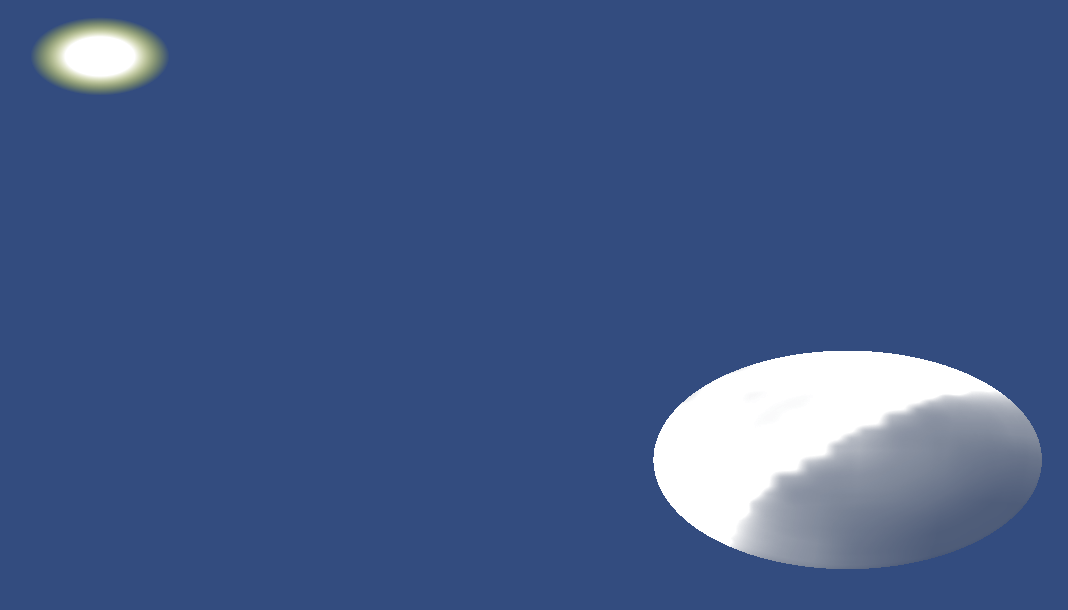
\includegraphics[width=\textwidth]{../res/conetrace.png}
\caption{Cone tracing results of a single billboard}
\end{figure}

Our cone trace method is fully paramterized. The user can change the number of ray march steps, the angle of cone's tip, the start offset of the cone along the ray, and an LOD offset. 

